\chapter{Partitional Clustering Background}
\label{cha:background}

\section{Summary}
\label{sec:summary-backgd}

In this chapter we first introduce the relevant terminology that is required
for much of the work presented in this thesis including metrics and
partitions.  We then review the field of partitional clustering including the
various criteria which have been developed, the computational complexity
issues associated with the clustering problem and finally various methods
which have been developed to perform partitional clustering.

\section{Datasets and metric spaces}
\label{sec:datas-metr-spac}

A dataset, in the most general sense, is simply a collection of objects.  For
now we will consider the collection to be a set, but later we will look at
some generalisations.

Let $\dset$ be a set.  It is important for many applications to be able to
compare objects in a set.  For this purpose we can define a function:
\begin{equation*}
  d \colon \dset \times \dset \to \mathbb{R}^{\geq 0}.
\end{equation*}
Such a function is called a \textit{dissimilarity on $\dset$}.  Whenever we
have, for any $x,y,z \in \dset$, that $d(x,y)>d(x,z)$, we interpret it as
``$x,y$ are more dissimilar than $x,z$''.

Examples of dissimilarities include Bregman divergences, which are
generalisations of Euclidean distance squared for objects in Euclidean space
\citep{banerjee2005clustering}, and the Kullback-Leibler divergence for
probability distributions \citep{kullback68information}.

Some dissimilarities are more useful than others.  One would generally expect
such a function to have the following two properties for all $x,y \in \dset$:
\begin{enumerate}
\item $d(x,y) = d(y,x)$ \quad (symmetry),
\item \label{item:distinct} $d(x,x) = 0$ \quad (identical elements are most
  similar).
\end{enumerate}
A dissimilarity on $\dset$ that satisfies these two properties is called a
\textit{distance on $\dset$}.  When we use a distance, objects are usually
said to be close or distant instead of similar or dissimilar.

Examples of distances include the Bhattacharyya distance
\citep{bhattacharyya43distance} and the \textit{single-linkage} distance that
we will see in Section~\ref{sec:set-metric}.

Two further properties that one may expect a dissimilarity to satisfy are, for
all $x,y,z \in \dset$:
\begin{enumerate}[resume]
\item \label{item:identity} $d(x,y) = 0$ only if $x=y$ \quad (identity of
  indiscernibles),
\item \label{item:tri-ineq} $d(x,y)+d(y,z) \geq d(x,z)$ \quad (triangle inequality).
\end{enumerate}
A distance on $\dset$ which satisfies all four properties is called a
\textit{metric on $\dset$}.  If $d$ is a metric on $\dset$ then the pair
$(\dset,d)$ is called a \textit{metric space}.

A metric is usually the most desirable and intuitive type of dissimilarity.
In the remainder of this section we review some of the common metrics used for
certain types of objects, namely Euclidean vectors, sequences, mixed vectors
and sets.

Metrics exist for many other types of objects including probability
distributions, for which metrics include the Hellinger distance and squared
Jensen-Shannon divergence \citep{endres03metric}.  It is also possible to
transform some dissimilarities into metrics, for example see
\citet[chap. 2.5]{everitt80}.  In Section~\ref{sec:comparing-partitions} we
look at metrics (and other measures) for comparing partitions and in
Chapter~\ref{cha:sum-squar-clust} we introduce our own metric.

\subsection{Euclidean space metrics}
\label{sec:eucl-space-metr}

Let $M$ be $m$-dimensional Euclidean space, $\mathbb{R}^m$.  For all
$\vec{x}=(x_1,x_2,\dotsc,x_m), \vec{y}=(y_1,y_2,\dotsc,y_m) \in M$, metrics on
$M$ include the familiar \textit{Euclidean distance} $\dissimdefn{E}$ defined
as:
\begin{equation*}
  d_E(\vec{x},\vec{y}) = \sqrt{\sum_{i=1}^{m} (x_i - y_i)^2},
\end{equation*}
the \textit{Manhattan distance} $\dissimdefn{M}$ defined as:
\begin{equation*}
  d_{M}(\vec{x},\vec{y}) = \sum_{i=1}^{m} |x_i - y_i|
\end{equation*}
and the \textit{Chebyshev distance} $\dissimdefn{C}$ defined as:
\begin{equation*}
  d_C(\vec{x},\vec{y}) = \max_{1 \leq i \leq m} |x_i - y_i|.
\end{equation*}
It should be noted that all three are special cases of the \textit{Minkowski
  distance} \citep{deza2009encyclopedia}, $\dissimdefn{I}$ defined as:
\begin{equation*}
  d_{I}(\vec{x},\vec{y}) = \left(\sum_{i=1}^{m} |x_i - y_i|^{p}\right)^{\prettyfrac{1}{p}}
\end{equation*}
for all $\vec{x}=(x_1,x_2,\dotsc,x_m), \vec{y}=(y_1,y_2,\dotsc,y_m) \in M$
where $p$ is the order.  For $p=1$, $d_I=d_M$, for $p=2$, $d_I=d_E$ and for
$\lim_{p \to \infty}$, $d_I=d_C$.

The Mahalanobis distance \citep{mahalanobis30distance} is a metric which is
equivalent to Euclidean distance on scaled principle components of the
dataset.  To make this more precise, let $\dset =
\{\vec{s}_1,\dotsc,\vec{s}_n\} \subset \mathbb{R}^m$, then the
\textit{covariance} of the $i$th and $j$th components in $\dset$ is defined
as:
\begin{equation*}
  S_{ij} = \frac{1}{n-1} \sum_{k=1}^{n} (s_{ki}-\bar{s}_i)(s_{kj}-\bar{s}_j),
\end{equation*}
where $s_{ki}$ means the $i$th component of the $k$th element and $\bar{s}_i$
means the mean of component $i$ across $\dset$.  In this context, components
are often called \textit{features} or \textit{fields}.  The covariance matrix
associated with $\dset$ is then the $m \times m$ matrix $S = [S_{ij}]$, which
is clearly symmetric.  The Mahalanobis distance, $d_{P} \colon \dset \times
\dset \to \mathbb{R}^{\geq 0}$, is then defined as:
\begin{equation*}
  d_{P}(\vec{x},\vec{y}) = \sqrt{(\vec{x}-\vec{y})S^{-1}(\vec{x}-\vec{y})^T},
\end{equation*}
for all $\vec{x},\vec{y} \in \dset$.

\subsection{Sequence space metrics}
\label{sec:sequ-space-metr}

Sequences are a frequently occurring type of object found in many areas such
as evolutionary biology and the analysis of natural language.  A well-known
metric on sequences of equal length is the \textit{Hamming distance}
\citep{hamming50errorcodes}.  The Hamming distance, for two sequences $x$ and
$y$ of equal length, is equal to the number of positions where $x$ and $y$
differ.

Another well-known metric, this time on sequences of arbitrary length, is the
Levenshtein distance \cite{levenshtein1965distance}.  The Levenshtein distance
is an edit distance, where the allowed edits are insertion, deletion and
substitution (for definitions, see \cite{levenshtein1966distanceEN}).  The
Levenshtein distance between two sequences $x$ and $y$ is the minimum number
of edits required to transform one sequence into the other.

\subsection{Mixed data metrics}
\label{sec:mixed-data-metrics}

Euclidean space consists of $m$-tuples of real numbers, where $m$ is some
positive integer.  This type of data is often called numerical data.  Another
type of data is categorical data, where the value of each object is one of a
fixed, usually small, number of categories, such as true and false or male and
female.

The simplest metric for categorical data is the \textit{overlap metric}, which
is also variously called the \textit{split metric}, \textit{discrete metric}
or \textit{$0/1$ metric}.  For a set, $\dset$, the overlap metric, $d_{O}
\colon \dset \times \dset \to \mathbb{R}^{\geq 0}$, is defined as:
\begin{equation*}
  d_O(x,y) =
  \begin{cases}
    0 & \text{if $x=y$,} \\
    1 & \text{otherwise,}
  \end{cases}
\end{equation*}
for all $x,y \in \dset$.

A frequently occurring type of data appearing in many areas is mixed data,
which consists of $m$-tuples with both numerical and categorical components.
Let $\dset$ be a set of such $m$-tuples.  The \textit{heterogeneous
  Euclidean-overlap metric}, $d_{H} \colon \dset \times \dset \to
\mathbb{R}^{\geq 0}$, uses normalised Euclidean distance on the numerical
components and the overlap metric on categorical components.  It is defined
as:
\begin{equation*}
  d_{H}(\vec{x},\vec{y}) = \sqrt{\sum_{i=1}^{m} d_{Hi}^2(x_i,y_i)},
\end{equation*}
for all $\vec{x}=(x_1,\dotsc,x_m),\vec{y}=(y_1,\dotsc,y_m) \in \dset$ where
\begin{equation*}
  d_{Hi}(x_i,y_i) =
  \begin{cases}
    d_O(x_i,y_i) & \text{if $i$ is a categorical component in $\dset$,} \\
    \displaystyle \frac{|x_i-y_i|}{range_i} & \text{otherwise,}
  \end{cases}
\end{equation*}
for all $1 \geq i \geq m$ where $range_i$ is the difference between maximum
and minimum observed values for component $i$ in $\dset$.

There also exist generalised Mahalanobis distances for mixed data, see for
example \citep{leon2005generalized}.

\subsection{Set metrics}
\label{sec:set-metric}

Metrics are also possible on more complex structures, like sets.  Throughout
this thesis we use a convention for naming dissimilarities: $d$ is used in
general, $\delta$ is used for dissimilarities on sets and, later, we will use
$\Delta$ for dissimilarities on partitions.  In this subsection we look at
some metrics on sets and in Section~\ref{sec:comparing-partitions} we will
look at dissimilarities on partitions.

\subsubsection{Symmetric difference}
\label{sec:symmetric-difference}

Let $\dset$ be a set and $2^\dset$ its powerset.  The cardinality of the
symmetric difference, $\delta_{\symdif} \colon 2^{\dset} \times 2^{\dset} \to
\mathbb{R}^{\geq 0}$ is a well-known metric on sets defined as:
\begin{equation*}
  \delta_{\symdif}(X,Y) = |X \symdif Y|,
\end{equation*}
for all $X,Y \in 2^{\dset}$.

\begin{figure}
  \centering
  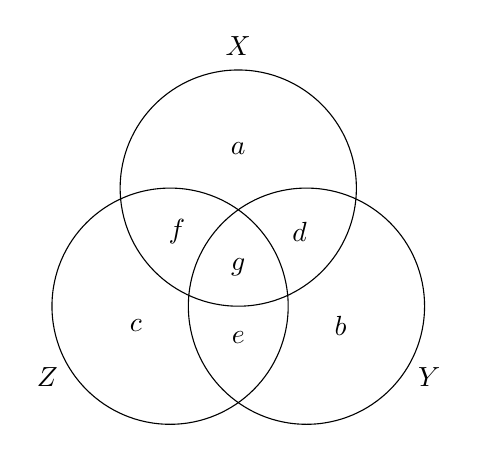
\begin{tikzpicture}
    % circles
    \draw (90:1) circle (1.5);
    \draw (210:1) circle (1.5);
    \draw (330:1) circle (1.5);

    % labels
    \node at (90:2.8) {$X$};
    \node at (330:2.8) {$Y$};
    \node at (210:2.8) {$Z$};
    
    \node at (90:1.5) {$a$};
    \node at (330:1.5) {$b$};
    \node at (210:1.5) {$c$};
    \node at (30:.9) {$d$};
    \node at (270:.9) {$e$};
    \node at (150:.9) {$f$};
    \node at (0:0) {$g$};
  \end{tikzpicture}
  \caption{Partition of $X \cup Y \cup Z$.  The quantities $a,b,c,d,e,f,g$
    represent the cardinalities of each disjoint set as shown.}
  \label{fig:partition}
\end{figure}

A related dissimilarity is the normalised symmetric difference,
$\delta_{\symdif} \colon 2^{\dset} \times 2^{\dset} \to \mathbb{R}^{\geq 0}$,
defined as:
\begin{equation*}
  \delta_{\symdif_n}(X,Y) =
  \begin{cases}
    \displaystyle \frac{|X \symdif Y|}{|X \cup Y|} & \text{if $X \cup Y \neq
      \emptyset$}, \\
    0 & \text{otherwise,}
  \end{cases}
\end{equation*}
for all $X,Y \in 2^{\dset}$.

\begin{thm}
  The normalised symmetric difference is a metric on $2^{\dset}$.
\end{thm}

The following proof was presented in \citep{yianilos91}, with some errors.  We
reproduce the proof here with the errors corrected.

\begin{proof}
  It is easy to see the function is nonnegative, symmetric and that
  $\delta_{\symdif_n}(X,Y)=0$ if and only if $X=Y$ for all $X,Y \in 2^{\dset}$
  so we will show that the triangle inequality holds which is:
  \begin{equation*}
    \frac{|X \symdif Y|}{|X \cup Y|} + \frac{|Y \symdif Z|}{|Y \cup Z|} \geq
    \frac{|X \symdif Z|}{|X \cup Y|}
  \end{equation*}
  or, equivalently:
  \begin{equation}
    \label{eq:tri-inequality}
    1 - \frac{|X \cap Y|}{|X \cup Y|} +
    1 - \frac{|Y \cap Z|}{|Y \cup Z|} \geq
    1 - \frac{|X \cap Z|}{|X \cup Z|}.
  \end{equation}

  We partition $X \cup Y \cup Z$ into disjoint subsets as shown in
  Figure~\ref{fig:partition} and let
  \begin{align*}
    a = |X \setminus (Y \cup Z)|,&\qquad
    b = |Y \setminus (X \cup Z)|,\\
    c = |Z \setminus (X \cup Y)|,&\qquad
    d = |(X \cap Y) \setminus Z|.\\
    e = |(Y \cap Z) \setminus X|.&\qquad
    f = |(Z \cap X) \setminus Y|.\\
    g = |X& \cap Y \cap Z|,
  \end{align*}
  and for convenience we let
  \begin{equation*}
    \xi  = |X \cup Y \cup Z|.
  \end{equation*}

  We can now write equation~(\ref{eq:tri-inequality}) as
  \begin{equation*}
    1 - \frac{d+g}{\xi -c} + 1 - \frac{e+g}{\xi -a} \geq 1 - \frac{f+g}{\xi -b}
  \end{equation*}
  which can be rewritten as
  \begin{equation*}
    \frac{d+g}{\xi -c} + \frac{e+g}{\xi -a} \leq \frac{f+g}{\xi -b} + 1.
  \end{equation*}

  Removing $b$ from the denominators on the LHS can only make the LHS
  greater, so it is sufficient to show that
  \begin{equation*}
    \frac{d+g}{\xi -b-c} + \frac{e+g}{\xi -a-b} \leq \frac{f+g}{\xi -b} + 1.
  \end{equation*}

  Now if we replace $1$ with $\frac{\xi -a-b-c}{\xi -a-b-c}$ on the RHS and add
  the fractions on the LHS we get
  \begin{multline*}
    \frac{(\xi -a-b)(d+g)+(\xi -b-c)(e+g)}{(\xi -b-c)(\xi -a-b)}\\
    \leq \frac{(\xi -a-b-c)(\xi -b)+(\xi -a-b-c)(f+g)}{(\xi -b)(\xi -a-b-c)}
  \end{multline*}
  which when we expand the denominators becomes
  \begin{multline*}
    \frac{(\xi -a-b)(d+g)+(\xi -b-c)(e+g)}{\xi ^2-\xi a-2\xi b-\xi c+ab+bc+b^2+ac}\\
    \leq \frac{(\xi -a-b-c)(\xi -b)+(\xi -a-b-c)(f+g)}{\xi ^2-\xi a-2\xi b-\xi c+ab+bc+b^2}.
  \end{multline*}
  Notice that the denominator on the LHS is equal to the denominator on the
  RHS with the addition of $ac$ so it cannot be less.  It is therefore
  sufficient to show that
  \begin{multline*}
    (\xi -a-b)(d+g)+(\xi -b-c)(e+g)\\
    \leq (\xi -a-b-c)(\xi -b)+(\xi -a-b-c)(f+g).
  \end{multline*}

  Starting with the LHS we have
  \begin{align*}
    &(\xi -a-b)(d+g)+(\xi -c-b)(e+g)\\
    &= (\xi -a-b-c)(d+g)+c(d+g)+(\xi -a-b-c)(e+g)+a(e+g)\\
    &\leq (\xi -a-b-c)(d+g)+c(\xi -a-b-c)\\
    &\qquad\qquad+(\xi -a-b-c)(e+g)+a(\xi -a-b-c)\\
    &= c(\xi -a-b-c)+(\xi -a-b-c)(d+e+g)\\
    &\qquad\qquad+g(\xi -a-b-c)+a(\xi -a-b-c)\\
    &\leq c(\xi -a-b-c)+(\xi -a-b-c)^2+g(\xi -a-b-c)+a(\xi -a-b-c)\\
    &= (\xi -a-b-c)(\xi -b)+g(\xi -a-b-c)\\
    &\leq (\xi -a-b-c)(\xi -b) + (f+g)(\xi -a-b-c).
  \end{align*}
\end{proof}

\subsubsection{Hausdorff distance}
\label{sec:hausdorff-distance}

\begin{figure}
  \centering
  \begin{tikzpicture}[
    ]

    \draw [dashed,faint] (-2.8em,0) ellipse (4em and 5em);
    \draw [dashed,faint] (2.8em,0) ellipse (5em and 4em);

    % set 1 primary markers
    \begin{scope}[xshift=-2.8em,scale=0.85]
      \foreach \theta in {0,30,...,330} {
        \pgfmathparse{(4*5)/sqrt((5*cos(\theta))^2+(4*sin(\theta))^2)}
        \node [setnode1] (1set\theta) at (\theta:\pgfmathresult em) {};
      }
    \end{scope}
    % set 2 markers
    \begin{scope}[xshift=-2.8em,scale=0.85]
      \foreach \theta in {0,30,330} {
        \pgfmathparse{(4*5)/sqrt((5*cos(\theta))^2+(4*sin(\theta))^2)}
        \node [setnode2] at (\theta:\pgfmathresult em) {};
      }
    \end{scope}

    % set 2 primary markers
    \begin{scope}[xshift=2.8em,scale=0.85]
      \foreach \theta in {0,30,...,330} {
        \pgfmathparse{(5*4)/sqrt((4*cos(\theta))^2+(5*sin(\theta))^2)}
        \node [setnode2] (2set\theta) at (\theta:\pgfmathresult em) {};
      }
    \end{scope}
    % set 1 markers
    \begin{scope}[xshift=2.8em,scale=0.85]
      \foreach \theta in {150,180,210} {
        \pgfmathparse{(5*4)/sqrt((4*cos(\theta))^2+(5*sin(\theta))^2)}
        \node [setnode1] at (\theta:\pgfmathresult em) {};
      }
    \end{scope}

    \draw [symdist] (2set0) -- node[auto,swap] {$d$} (1set0);

    % labels
    \node at (-6em,4em) {$X$};
    \node at (6em,4em) {$Y$};
  \end{tikzpicture}
  \caption{$X$ and $Y$ are sets with elements labelled by \tikzuptriangle ~and
    \tikzupdtriangle ~respectively.  Elements in both sets are labelled with
    \tikzbotriangle .  The Hausdorff distance between $X$ and $Y$ is,
    informally, the greatest distance one must travel if starting from a point
    in one set and travelling to the closest point in the other.  This
    distance is marked by $d$ in the diagram.}
  \label{fig:haussdorf}
\end{figure}

Let $(M,d)$ be a metric space and $\mathcal{M}=2^M \setminus \{\emptyset\}$.
The Hausdorff distance, $\delta_{H} \colon \mathcal{M} \times \mathcal{M} \to
\mathbb{R}^{\geq 0}$, is defined as:
\begin{equation*}
  \delta_{H}(X,Y) = \max\left(\max_{x \in X} \min_{y \in Y} d(x,y),
                             \max_{y \in Y} \min_{x \in X} d(x,y)\right), 
\end{equation*}
for all $X,Y \in \mathcal{M}$.  The Hausdorff distance is a metric on
$\mathcal{M}$ \citep{braun2003geometry}.  This distance is illustrated in
Figure~\ref{fig:haussdorf} by showing the Hausdorff distance between two sets
with elements in a metric space.  In Chapter~\ref{cha:sum-squar-clust} we
present a new metric on $\mathcal{M}$.

\subsubsection{Linkage functions}
\label{sec:linkage-functions}

We conclude by remarking that the linkage functions, which are used in
hierarchical clustering, the topic of Section~\ref{sec:hier-clust-meth}, are
not generally metrics.  For a metric space, $(M,d)$, and $\mathcal{M}=2^M
\setminus \emptyset$, the \textit{single-linkage distance}, $\delta_{SL}
\colon \mathcal{M} \times \mathcal{M} \to \mathbb{R}^{\geq 0}$ is defined as:
\begin{equation*}
  \delta_{SL}(X,Y) = \min_{x \in X, y \in Y} d(x,y),
\end{equation*}
for all $X,Y \in \mathcal{M}$.  While single-linkage is a simple and intuitive
distance between sets, it is not a metric since distinct sets can have a
distance of zero.  The \textit{complete-linkage} and \textit{average-linkage}
dissimilarities are, in fact, not even distances.  These measures will be
discussed further in Section~\ref{sec:hier-clust-meth}.

% \subsection{Multiset datasets}
% \label{sec:multiset-datasets}

% It is tempting to think of a dataset and a metric defined on its elements as a
% metric space, but this is not necessarily correct.  The reason is that,
% contrary to the name, a dataset is not usually a set but a multiset.  Consider
% a dataset consisting of only the heights of some population of humans.
% Depending on the precision of the measurements taken, it would generally be
% expected that multiple subjects share the same height.  In order to have these
% observations in a set, some unique integer---an experiment number, say---would
% need to be attached to each observation.  But then the metric condition that
% $d(x,y)=0$ only if $x=y$ would be violated---in fact we would have only a
% \textit{pseudometric}.  We can get a proper metric if we define an equivalence
% relation $x \sim y$ if $d(x,y)=0$.  Then $(\dset/\sim,d)$ is a metric space.

% Most of the time we do not need to worry about this.  From now on a dataset,
% $\dset$, will implicitly mean $\dset/\sim$ as defined above unless stated
% otherwise.  Occasionally. though, it will be useful or necessary to consider
% the multiset $(\dset,\mu_{\dset})$ where $\dset$ is the underlying set, and
% $\mu_{\dset} \colon \dset \to \mathbb{N}_1$---a map from $\dset$ to the
% (nonzero) natural numbers---is called the membership function and tells us how
% many times an element appears in the multiset.

% A further generalisation is then possible: we can relax the definition of the
% membership function to $\mu_{\dset} \colon \dset \to \mathbb{R}_1$---a map
% from $\dset$ to the positive real numbers.  The dataset is then a fuzzy
% multiset.  Such datasets have been used in document clustering applications,
% for example in \citep{miyamoto2003information}, where objects can appear
% multiple times with a certain probability attached.  If the membership
% function if $\mu_{\dset} \colon \dset \to \mathbb{R}_1 \cap [0,1]$ then
% $(\dset,\mu_{\dset})$ is called a fuzzy set
% \citep{zadeh1965fuzzy,gottwald2010fuzzy}.

\section{Partitions}
\label{sec:partitions}

In this section we look at the properties of partitions of sets, how we can
compare partitions and how we can find partitions.  Throughout, we assume that
$n > 0$ and refer to a set of $n$ elements as an \textit{$n$-set}.

\subsection{The space of partitions}
\label{sec:space-partitions}

Given an $n$-set $\dset$, a $k$-partition $\clus = \{C_1,C_2,\dotsc,C_k\}$ of
$\dset$ is a set of $k \in \{1,\dotsc,n\}$ nonempty, pairwise-disjoint subsets
of $\dset$ such that $C_1 \cup C_2 \cup \dotsb \cup C_k = \dset$.  Following
common practice, we will refer to the elements of $\clus$ as
\textit{clusters}.

\begin{figure}
  \centering
  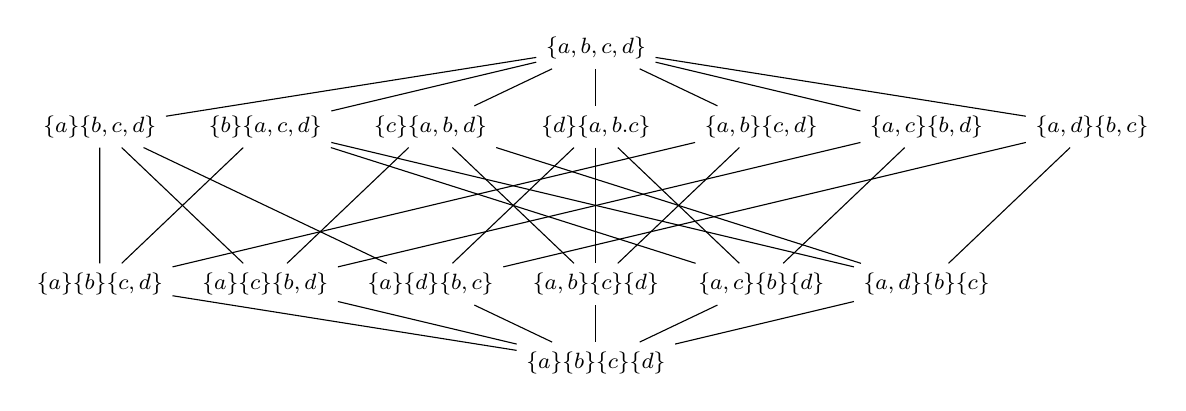
\begin{tikzpicture}[
    xscale=2.1, font=\footnotesize]

    % vertices
    
    \node (0) at (0,0) {$\{a,b,c,d\}$};

    \node (10) at (-3,-1) {$\{a\}\{b,c,d\}$};
    \node (11) at (-2,-1) {$\{b\}\{a,c,d\}$};
    \node (12) at (-1,-1) {$\{c\}\{a,b,d\}$};
    \node (13) at (0,-1) {$\{d\}\{a,b.c\}$};
    \node (14) at (1,-1) {$\{a,b\}\{c,d\}$};
    \node (15) at (2,-1) {$\{a,c\}\{b,d\}$};
    \node (16) at (3,-1) {$\{a,d\}\{b,c\}$};

    \node (20) at (-3,-3) {$\{a\}\{b\}\{c,d\}$};
    \node (21) at (-2,-3) {$\{a\}\{c\}\{b,d\}$};
    \node (22) at (-1,-3) {$\{a\}\{d\}\{b,c\}$};
    \node (23) at (0,-3) {$\{a,b\}\{c\}\{d\}$};
    \node (24) at (1,-3) {$\{a,c\}\{b\}\{d\}$};
    \node (25) at (2,-3) {$\{a,d\}\{b\}\{c\}$};

    \node (3) at (0,-4) {$\{a\}\{b\}\{c\}\{d\}$};

    % edges

    \draw (0) to (10);
    \draw (0) to (11);
    \draw (0) to (12);
    \draw (0) to (13);
    \draw (0) to (14);
    \draw (0) to (15);
    \draw (0) to (16);

    \draw (10) to (20);
    \draw (10) to (21);
    \draw (10) to (22);
    \draw (11) to (20);
    \draw (11) to (24);
    \draw (11) to (25);
    \draw (12) to (21);
    \draw (12) to (23);
    \draw (12) to (25);
    \draw (13) to (22);
    \draw (13) to (23);
    \draw (13) to (24);
    \draw (14) to (20);
    \draw (14) to (23);
    \draw (15) to (21);
    \draw (15) to (24);
    \draw (16) to (22);
    \draw (16) to (25);

    \draw (20) to (3);
    \draw (21) to (3);
    \draw (22) to (3);
    \draw (23) to (3);
    \draw (24) to (3);
    \draw (25) to (3);
  \end{tikzpicture}
  \caption{The Hasse diagram of the lattice of partitions of a set,
    $\dset=\{a,b,c,d\}$ \citep{meila-2005}.  Each vertex in the graph is a
    partition $\{C_1,\dotsc,C_k\}$ of $\dset$ which we denote by
    $C_1,\dotsc,C_k$ for clarity.}
  \label{fig:lattice}
\end{figure}

Let $\parts_{\dset}$ be the set of all partitions of $\dset$ and $\clus,\clus'
\in \parts_{\dset}$.  The partition $\clus$ is called a \textit{refinement} of
$\clus'$ if every element of $\clus$ is a subset of some element of $\clus'$.
We can then say that $\clus$ is \textit{finer-than-or-equal-to} $\clus'$,
which we notate $\clus \leq \clus'$ (or that $\clus'$ is
\textit{coarser-than-or-equal-to} $\clus$).  The relation $\leq$ imposes a
partial order on the elements of $\parts_{\dset}$.

The partially-ordered set $(\parts_{\dset},\leq)$ is called the
\textit{lattice of partitions} and can be represented in terms of a graph
called the \textit{Hasse diagram} associated with $\parts_{\dset}$.  The
vertex set of that graph is $\parts_{\dset}$ and its arc set consists of the
pairs $(\clus_1,\clus_2) \in \parts_{\dset} \times \parts_{\dset}$ such that
$\clus_2 < \clus_1$ and there exists no $\clus_3 \in \parts_{\dset}$ such that
$\clus_2 < \clus_3 < \clus_1$.  Informally, this means that $\clus_2$ can be
obtained by bisecting one cluster of $\clus_1$.

The Hasse diagram of the set $\dset = \{a,b,c,d\}$ is presented in
Figure~\ref{fig:lattice}.  The partition at the top is the coarsest partition
(a 1-partition) and the partition at the bottom is the finest partition (an
$n$-partition).

As this example suggests, a set can potentially support a very large number of
partitions.  For an $n$-set $\dset$ the cardinality of $\parts_{\dset}$ is
given by the \textit{Bell number} $B_n$
\citep{bell1934exponential,stanley2000enumerative} where $B_0=1$ and
\begin{equation*}
  B_n = \sum_{l=0}^{n-1} B_l \binom{n-1}{l} \qquad \text{for $n \geq 1$}.
\end{equation*}
Alternatively, $B_n$ is given by Dobi\'{n}ski's formula
\citep{dobinski1877summation}:
\begin{equation*}
  B_n = \frac{1}{e} \sum_{l=0}^{\infty} \frac{l^n}{l!} \qquad \text{for $n
    \geq 0$}.
\end{equation*}
We illustrate the growth of the Bell number in Table~\ref{tab:bell-number}.

\begin{table}
  \centering
  \begin{tabular}{rr}
    \toprule
    $n$ & $B_n$ \\
    \midrule
    5 & 52 \\
    10 & 115,975 \\
    15 & 1,382,958,545 \\
    20 & $5.17 \times 10^{13}$ \\
    25 & $4.64 \times 10^{18}$ \\
    \bottomrule
  \end{tabular}
  \caption{The value of the Bell number, $B_n$, for some selected values of
    $n$.  The value of $B_n$ is equivalent to the number of possible
    partitions of an $n$ element set.}
  \label{tab:bell-number}
\end{table}

\subsubsection{Fuzzy partitions}
\label{sec:fuzzy-partitions}

Partitions can be generalised to fuzzy partitions by letting the clusters be
fuzzy sets.  Fuzzy sets are collections of objects where each member of a
collection has a grade of membership associated to it \citep{zadeh1965fuzzy}.
Sets are a special case where the grades of membership are binary---objects
are either members of a set or they are not.  Fuzzy sets and partitions have
many applications including classification of data in the natural sciences
where membership is not precisely defined.

Formally, a fuzzy set is an ordered pair $(C,\mu_{C})$ consisting of an
underlying set $C$ and a membership function $\mu_{C} \colon C \to [0,1]$.
For some fuzzy set $(C,\mu_C)$ and element $x \in C$ $\mu_C(x) = 1$ means $x$
is a full member, $\mu_C(x) = 0$ means $x$ is not a member and $0 < \mu_C(x) <
1$ means $x$ is a fuzzy member.  If $\mu_C(x) = 0$ or $1$ for all $x \in C$
then the object is called by contrast a \textit{crisp set} and may be handled
by ordinary set theory \cite{zadeh1965fuzzy,klir1995fuzzy}.

A \textit{$k$-fuzzy-partition} of an $n$-set $\dset$ is a set of $k \in
\{1,\dotsc,n\}$ fuzzy sets: \[\{(C_1,\mu_1),(C_2,\mu_2),\dotsc,(C_k,\mu_k)\}\]
where $C_1 \cup \dotsb \cup C_k = \dset$, $C_i \neq \emptyset$ for all $i \in
\{1,\dotsc,k\}$ and $\sum_{i=1}^{k} \mu_i(x) = 1$ for all $x \in \dset$.  Note
that the underlying sets of the fuzzy sets $(C_i,\mu_i)$ are not necessarily
pairwise disjoint, so elements can belong to more than one cluster.

\subsection{Comparing partitions}
\label{sec:comparing-partitions}

An attractive way to find partitions of a set is by means of a partitional
clustering method.  Many methods exist---we will review some in
Section~\ref{sec:part-clust-algor}---and, depending on their respective
approach to the problem, they all tend to produce different partitions.  To
further complicate matters, some methods are nondeterministic so can
potentially produce different partitions each time they are used.

For the purposes of comparing and assessing clustering methods it is therefore
useful to be able to compare partitions.  Many measures have been devised for
this purpose, including similarity measures and dissimilarity measures, of
which some are metrics.  Existing methods fall into four main categories; for
two partitions $\clus_1$ and $\clus_2$ of a set $\dset$, these are:
\begin{description}
\item[Pair counting] which measures the agreement and disagreement between
  $\clus_1$ and $\clus_2$ by means of counting pairs of element in $\dset$,
\item[Set matching] which ``matches'' clusters in $\clus_1$ with clusters in
  $\clus_2$ and measures the similarity between matched sets,
\item[Information theoretic] which uses information theory to measure the
  information and mutual information contained in $\clus_1$ and $\clus_2$,
\item[Density profile] which takes into account the values of the data when
  computing the measure.
\end{description}

We will review measures belonging to the first three categories in this
section.  The fourth category consists of a single measure called ADCO which
we will analyse in Chapter~\ref{cha:sum-squar-clust}.

To be able to describe the measures in detail, we need to introduce some more
terminology.  Let $\dset = \{x_1,x_2,\dotsc,x_n\}$ be an $n$-set with $n \geq
2$ and again, as before, let $\clus_1 = \{C_{11},C_{12},\dotsc,C_{1k}\}$ and
$\clus_2 = \{C_{21},C_{22},\dotsc,C_{2k'}\}$ be two partitions of $\dset$ with
$k$ and $k'$ clusters, respectively.  We denote, for some $x \in \dset$, and a
partition, $\clus$, of $\dset$, the cluster in $\clus$ that contains $x$ by
$\clus(x)$.  The \textit{confusion matrix} associated with $\clus_1$ and
$\clus_2$ is the $k \times k'$ matrix $[n_{ij}]$ where $n_{ij} = |C_{1i} \cap
C_{2j}|$.  It is used for the calculation of both pair counting and set
matching measures.

To illustrate these definitions and the comparison measures we review below,
we will use two example partitions $\clus^*_1$ and $\clus^*_2$ of the set
$\dset^* = \{1,\dotsc,9\}$ throughout this section:
\begin{equation}
  \label{eq:example-parts}
  \clus^*_1 = \{C^*_{11},C^*_{12},C^*_{13}\},\qquad
  \clus^*_2 = \{C^*_{21},C^*_{22},C^*_{23},C^*_{24}\}
\end{equation}
where
\begin{align*}
  C^*_{11}&=\{1,2,3\},\quad C^*_{12}=\{4,5,6\},\quad C^*_{13}\{7,8,9\} \quad \text{and}\\
  C^*_{21}&=\{1,4\},\quad C^*_{22}=\{2,3,6\},\quad C^*_{23}=\{5,8\},\quad C^*_{24}\{7,9\}.
\end{align*}
Then, for example, we have $\clus^*_1(3) = C^*_{11}$, and the confusion matrix
associated with $\clus^*_1$ and $\clus^*_2$ is:
\begin{equation*}
  [n_{ij}]^*=\left[
  \begin{matrix}
    1 & 2 & 0 & 0 \\
    1 & 1 & 1 & 0 \\
    0 & 0 & 1 & 2
  \end{matrix}
  \right]
\end{equation*}

\subsubsection{Pair counting}
\label{sec:pair-counting}

There are $\binom{n}{2}$ distinct pairs of elements in $\dset$.  For each
distinct pair $(a,b) \in \dset \times \dset$ one of the following is true:
\begin{align*}
\clus_1(a)=\clus_1(b) &\text{ and } \clus_2(a)=\clus_2(b),\\
\clus_1(a)\neq \clus_1(b) &\text{ and } \clus_2(a)\neq \clus_2(b),\\
\clus_1(a)=\clus_1(b) &\text{ and } \clus_2(a)\neq \clus_2(b),\\
\clus_1(a)\neq \clus_1(b) &\text{ and } \clus_2(a)=\clus_2(b).
\end{align*}
Counting the number of element in each category gives us four counts which are
defined formally as:
\begin{align*}
  N_{11} &= |\{(a,b) \in \dset \times \dset \colon
              \clus_1(a)=\clus_1(b) \text{ and } \clus_2(a)=\clus_2(b)
            \}|, \\
  N_{00} &= |\{(a,b) \in \dset \times \dset \colon
              \clus_1(a)\neq\clus_1(b) \text{ and } \clus_2(a)\neq\clus_2(b)
            \}|, \\
  N_{10} &= |\{(a,b) \in \dset \times \dset \colon
              \clus_1(a)=\clus_1(b) \text{ and } \clus_2(a)\neq\clus_2(b)
            \}|, \\
  N_{01} &= |\{(a,b) \in \dset \times \dset \colon
              \clus_1(a)\neq\clus_1(b) \text{ and } \clus_2(a)=\clus_2(b)
            \}|.
\end{align*}
The size of $N_{11}$ and $N_{00}$ are considered to be measurements of
\textit{agreement} between $\clus_1$ and $\clus_2$, while $N_{10}$ and
$N_{01}$ are considered measurements of \textit{disagreement}.

The measures based on pair counting can all be expressed in terms of these
four counts.  Clearly \[N_{11}+N_{00}+N_{10}+N_{01} = \binom{n}{2}\] is always
satisfied.  The quantities $N_{11},N_{00},N_{10}$ and $N_{01}$ can all be
obtained from the confusion matrix using the following formul\ae
\citep{hubert-arabie-1985}:
\begin{align*}
  N_{11} &= \frac{1}{2} \sum_{i=1}^{k} \sum_{j=1}^{k'} n_{ij}(n_{ij}-1),\\
  N_{00} &= \frac{1}{2} \left(n^2 + \sum_{i=1}^{k} \sum_{j=1}^{k'} n_{ij}^2
                             - \sum_{i=1}^{k}
                                \left(\sum_{j=1}^{k'} n_{ij} \right)^2
                             - \sum_{j=1}^{k'}
                                \left(\sum_{i=1}^{k} n_{ij} \right)^2
                       \right),\\
  N_{10} &= \frac{1}{2} \left(\sum_{i=1}^{k}
                              \left(\sum_{j=1}^{k'} n_{ij} \right)^2
                             - \sum_{i=1}^{k} \sum_{j=1}^{k'} n_{ij}^2
                       \right),\\
  N_{01} &= \frac{1}{2} \left(\sum_{j=1}^{k'}
                              \left(\sum_{i=1}^{k} n_{ij} \right)^2
                             - \sum_{i=1}^{k} \sum_{j=1}^{k'} n_{ij}^2
                       \right).
\end{align*}
The four counts for our example partitions $\clus^*_1$ and $\clus^*_2$ are:
\begin{equation*}
  N_{11} = 2,\quad
  N_{00} = 23,\quad
  N_{10} = 7,\quad
  N_{01} = 4.
\end{equation*}

One of the simplest pair counting measures between $\clus_1$ and $\clus_2$ is
the widely-used \textit{Rand index} $\partcomparen{R}$ introduced in
\citep{rand-1971} and defined as:
\begin{equation*}
\partcompare{R} = \frac{(N_{11}+N_{00})}{\binom{n}{2}}.
\end{equation*}
The Rand index is a similarity measure with a lower bound of 0 and an upper
bound of 1.  \citet{hubert-arabie-1985} use the following variation:
\[\partcompare{HA} = (N_{11}+N_{00}-N_{10}-N_{01})/\binom{n}{2}.\]

\citet{wallace-1983} introduced two asymmetric measures for comparing
$\clus_1$ and $\clus_2$ defined as:
\begin{equation*}
  \mathcal{W}_{I}(\clus_1,\clus_2) =
  \frac{N_{11}}{\sum_{i=1}^{k} |C_{i1}|(|C_{1i}|-1)/2},
\end{equation*}
and
\begin{equation*}
  \mathcal{W}_{II}(\clus_1,\clus_2) =
  \frac{N_{11}}{\sum_{j=1}^{k'} |C_{2j}|(|C_{2j}|-1)/2}.
\end{equation*}
$\mathcal{W}_{I}$ and $\mathcal{W}_{II}$ represent the probabilities that, for
a pair of elements $(a,b) \in \dset \times \dset$ with
$\clus_1(a)=\clus_1(b)$, we also have $\clus_2(a)=\clus_2(b)$, and vice versa.
A symmetric similarity measure for $\clus_1$ and $\clus_2$ can be obtained by
taking the geometric mean of the Wallace measures:
\begin{equation*}
  \partcompare{F} = \sqrt{\mathcal{W}_{I}(\clus_1,\clus_2)
                          \mathcal{W}_{II}(\clus_1,\clus_2)}.
\end{equation*}
This measure was also introduced independently by Fowlkes and Mallows in
\citep{fowlkes-mallows-1983}.

The \textit{Jaccard coefficient} $\partcomparen{J}$ is another widely-used
similarity measure and is defined, for $\clus_1$ and $\clus_2$, as:
\begin{equation*}
  \partcompare{J} = \frac{N_{11}}{N_{10}+N_{01}+N_{11}}.
\end{equation*}

It should be noted that all measures reviewed so far are similarity measures.
The \textit{Mirkin metric} $\partcomparen{M}$ for measuring dissimilarity
between $\clus_1$ and $\clus_2$ was originally introduced in
\citep{mirkin1996mathematical} and is defined as
\begin{equation*}
  \partcompare{M} = \sum_{i=1}^{k} |C_{1i}|^2 +
                    \sum_{j=1}^{k'} |C_{1j}|^2 +
                    2\sum_{i=1}^{k}\sum_{j=1}^{k'} n_{ij}^2,
\end{equation*}
where $[n_{ij}]$ again denotes the confusion matrix associated with $\clus_1$
and $\clus_2$.  As it turns out, \[\partcompare{M}=2(N_{10}+N_{01}).\] The
closely related measure: \[\partcompare{AB}=(N_{10}+N_{01})/\binom{n}{2}\] is
also a metric on $\parts_{\dset}$ and was used by
\citet{mirkin1970measurement} and \citet{arabie1973multidimensional}.

\begin{table}
  \centering
  \begin{tabular}{lr}
    \toprule
    Name & Measure \\
    \midrule
    Rand index          & $\partcomparest{R} \approx 0.694$ \\
    Wallace measures    & $\mathcal{W}_{I}(\clus^*_1,\clus^*_2) \approx 0.222$ \\
                        & $\mathcal{W}_{II}(\clus^*_1,\clus^*_2) \approx 0.333$ \\
    Fowlkes \& Mallows  & $\partcomparest{F} \approx 0.272$ \\
    Jaccard coefficient & $\partcomparest{J} \approx 0.154$ \\
    Merkin metric       & $\partcomparest{M} = 22.00$ \\
    \bottomrule
  \end{tabular}
  \caption{Various pair counting based measures applied to the example
    partitions $\clus^*_1$ and $\clus^*_2$~\eqref{eq:example-parts}.}
  \label{tab:pair-counting-comparison}
\end{table}

The values of the reviewed pair counting measures when applied to $\clus^*_1$
and $\clus^*_2$ are given in Table~\ref{tab:pair-counting-comparison}.

\subsubsection{Set matching}
\label{sec:set-matching}

Set matching measures for partitions $\clus_1$ and $\clus_2$ are based on
comparisons between matched pairs of clusters.  Each pair to be compared
consists of one element of $\clus_1$ and one of $\clus_2$.  All of the
measures that we review here are based on the confusion matrix, meaning that
they use the cardinality of the intersection between two clusters as a
similarity measure.  The differences between the measures are essentially due
to the way that they find the matched pairs of clusters for comparison.

As before, let $\dset$ be an $n$-set and let $\clus_1 =
\{C_{11},\dotsc,C_{1k}\}$ and $\clus_2 = \{C_{21},\dotsc,C_{1k'}\}$, where
$k,k' \geq 1$, denote two partitions of $\dset$.  Also assume, without loss of
generality, that $k' \geq k$.  Then, a \textit{matching} between $\clus_1$ and
$\clus_2$ is a function $\sigma \colon \{1,\dotsc,k\} \to \{1,\dotsc,k'\}$.

\begin{figure}
  \centering
  \begin{tikzpicture}[
    % >=stealth,
    % clus/.style={circle,draw=black,inner sep=0,minimum size=5mm},
    % dist/.style={->,shorten >=2pt},
    % faint/.style={dist,gray!50},
    nonmatch/.style={dist,faint},
    match/.style={dist,black}
    ]

    \node [clus] (c11) at (0,1) {$C_{11}$};
    \node [clus] (c12) at (0,0) {$C_{12}$};
    \node [clus] (c13) at (0,-1) {$C_{13}$};

    \node [clus] (c21) at (2,1.5) {$C_{21}$};
    \node [clus] (c22) at (2,.5) {$C_{22}$};
    \node [clus] (c23) at (2,-.5) {$C_{23}$};
    \node [clus] (c24) at (2,-1.5) {$C_{24}$};

    % join them all
    \foreach \x in {1,2,3} {
      \foreach \y in {1,2,3,4} {
        \draw [nonmatch] (c1\x) to (c2\y);
      }
    }

    % matches
    \draw [match] (c11) to (c22);
    \draw [match] (c12) to (c23);
    \draw [match] (c13) to (c21);
  \end{tikzpicture}
  \caption{The clusters belonging to two partitions $\{C_{11},\dotsc,C_{13}\}$
    and $\{C_{21},\dotsc,C_{24}\}$ are shown with all similarities between
    pairs shown in grey.  The black lines represent one possible matching
    between the clusters.  In this case, the matching is an injection.}
  \label{fig:matching}
\end{figure}

\citet{meila-2001} introduced a set matching measure for measuring the
similarity between $\clus_1$ and $\clus_2$.  It finds a matching $\sigma$
using the following heuristic: let $[n_{ij}]$ be the $k \times k'$ confusion
matrix associated with $\clus_1$ and $\clus_2$.  Compute $n_{ab} = \argmax
\{n_{ij} \colon 1 \leq i \leq k, 1 \leq j \leq k'\}$ and put $\sigma(a) \gets
b$.  Repeat the process for the $(k-1) \times (k'-1)$ submatrix obtained by
deleting row $a$ and column $b$, and so on until $k$ matches have been made.
This process clearly finds an injection for $\sigma$ and then the similarity
of $\clus_1$ and $\clus_2$ based on that matching is:
\begin{equation*}
  \partcompare{H} = \frac{1}{n} \sum_{i=1}^{k} n_{i \sigma(i)}.
\end{equation*}

A second similarity measure on $\parts_{\dset}$, denoted $\partcomparen{L}$
and introduced by \citet{larsen-aone-1999} simply computes a maximal match for
each cluster in $\clus_1$ and $\clus_2$:
\begin{equation*}
  \partcompare{L} = \frac{1}{k} \sum_{i=1}^{k} \max_{1 \leq j \leq k'}
                                             \frac{2n_{ij}}{|C_{1i}|+|C_{2j}|}.
\end{equation*}

A dissimilarity measure $\partcomparen{V}$, which is a metric on
$\parts_{\dset}$, was introduced by \citet{van-dongen-2000}.  This measure,
again, computes maximal matches for each cluster in $\clus_1$ and $\clus_2$:
\begin{equation*}
  \partcompare{V} = 2n - \sum_{i=1}^{k} \max_{1 \leq j \leq k'} n_{ij}
                         \sum_{j=1}^{k'} \max_{1 \leq i \leq k} n_{ij}.
\end{equation*}

A second metric on $\parts_{\dset}$ denoted by $\partcomparen{CE}$ is due to
\citet{meila-2005} and is known by the name \textit{classification error}.
Like $\partcomparen{H}$, this measure computes an injection for $\sigma$, but
instead of using a heuristic finds a globally optimal injection in the set
$S_k$ of all possible injections from $\{1,\dotsc,k\}$ to $\{1,\dotsc,k'\}$:
\begin{equation*}
  \partcompare{CE} = 1 - \frac{1}{n} \max_{\sigma \in S_k}
                                     \sum_{i=1}^{k} n_{i \sigma(i)}.
\end{equation*}
Note that the injection, $\sigma$, can be found in polynomial time.  Also,
\[\partcompare{CE} \leq 1\] for all partitions $\clus_1$ and $\clus_2$ of
$\dset$.  The values of the set matching measures when applied to our example
partitions $\clus^*_1$ and $\clus^*_2$ are given in
Table~\ref{tab:set-matching-comparison}.

\begin{table}
  \centering
  \begin{tabular}{lr}
    \toprule
    Name & Measure \\
    \midrule
    Meilă \& Heckerman   & $\partcomparest{H} \approx 0.556$ \\
    Larsen \& Aone       & $\partcomparest{L} \approx 0.622$ \\
    Van Dongen metric    & $\partcomparest{V} = 7.000$ \\
    Classification Error & $\partcomparest{CE} \approx 0.445$ \\
    
    \bottomrule
  \end{tabular}
  \caption{Various set matching based measures applied to the example
    partitions $\clus^*_1$ and $\clus^*_2$~\eqref{eq:example-parts}.}
  \label{tab:set-matching-comparison}
\end{table}

\citet{meila-2007} and \citet{bae2010comparison} point out that all of these
measures suffer from the so-called ``problem of matching'' which we will now
illustrate.  Given a partition $\clus=\{C_1,\dotsc,C_k\}$ with $k\geq 2$
equally sized clusters, we can obtain a partition $\clus'$ from $\clus$ by
moving a fraction $f$ of the objects from each cluster $C_{i}$ to $C_{i+1}$,
with the indices taken$\mod k$.  We can obtain a further partition $\clus''$
from $\clus$ by taking the same fraction from each cluster in $C \in \clus$
and distributing the objects evenly among all other clusters in $\clus
\setminus \{C\}$.  Our intuition would be that the similarity between $\clus$
and $\clus'$ is not the same as the similarity between $\clus$ and $\clus''$.
However,
\begin{align*}
  \partcomparep{H} = \partcomparepp{H},&\quad
  \partcomparep{L} = \partcomparepp{L},\\
  \partcomparep{V} = \partcomparepp{V},&\quad
  \partcomparep{CE} = \partcomparepp{CE}
\end{align*}
whenever $0< f < 1/2$.

To give a numerical example, let $\dset = \{1,\dotsc,15\}$,
\begin{equation*}
  \clus = \{\{1,2,3,4,5\},\{6,7,8,9,10\},\{11,12,13,14,15\}\}
\end{equation*}
be a partition of $\dset$ and $f = 2/5$.  Then
\begin{equation*}
\clus' = \{\{1,2,3,14,15\},\{6,7,8,4,5\},\{11,12,13,9,10\}\}
\end{equation*}
and
\begin{equation*}
\clus'' = \{\{1,2,3,9,14\},\{6,7,8,4,15\},\{11,12,13,5,10\}\}
\end{equation*}
are partitions of $\dset$ obtained from $\clus$ as described above.  In this
case we have
\begin{align*}
  \partcomparep{H} = \partcomparepp{H} = 3/5,&\quad
  \partcomparep{L} = \partcomparepp{L} = 3/5,\\
  \partcomparep{V} = \partcomparepp{V} = 12,&\quad
  \partcomparep{CE} = \partcomparepp{CE} = 2/5.
\end{align*}

\subsubsection{Information theoretic}
\label{sec:inform-theor}

Two measures which use information theory are \textit{Normalized Mutual
  Information} \citep{fred-jain-2003} and \textit{Variation of Information}
\citep{meila-2007}.  For the remainder of this section we will focus on the
latter and refer the reader to \citep{fred-jain-2003} for details on the
former.

Variation of Information is based on both how much information is contained in
each partition and how much information one partition contains about the other
(their mutual information).

Let $\clus = \{C_{1},\dotsc,C_{k}\}$, where $k \geq 1$, be partition of an
$n$-set $\dset$.  Then the \textit{information} contained in $\clus$ is
measured by:
\begin{equation}
  \label{eq:entropy}
  H(\clus) = -\sum_{i=1}^{k} P_{\clus}(i) \log_b P_{\clus}(i),
\end{equation}
where
\begin{equation*}
  P_{\clus}(i) = \frac{|C_{i}|}{k}, \qquad \text{for $i = 1,\dotsc,k$}.
\end{equation*}
Informally, $P_1(i)$, is the probability that an object picked randomly from
$\dset$ is in cluster $C_{1i}$.  This measure is sometimes called
\textit{entropy}.  The base of the logarithm determines the unit of
information; for example, the bases $b=2,b=e$ and $b=10$ give the information
in so-called \textit{bits}, \textit{nits} and \textit{Hartleys}, respectively
\citep[see][]{kullback68information}.

Now, with $\clus_1 = \{C_{11},\dotsc,C_{1k}\}$ and $\clus_2 =
\{C_{21},\dotsc,C_{1k'}\}$, where $k,k' \geq 1$, the mutual information,
$I(\clus_1,\clus_2)$, between $\clus_1$ and $\clus_2$ is given by:
\begin{equation}
  \label{eq:mutualinf}
  I(\clus_1,\clus_2) = \sum_{i=1}^{k} \sum_{i=1}^{k'}
  P_{12}(i,j) \log_b \frac{P_{12}(i,j)}{P_{\clus_1}(i)P_{\clus_2}(j)},
\end{equation}
where
\begin{equation*}
  P_{12}(i,j) = \frac{|C_{1i} \cap C_{2j}|}{n}, \qquad \text{for $i =
    1,\dotsc,k,j = 1,\dotsc,k'$}.
\end{equation*}
Informally, $P_{12}(i,j)$ is the probability that an object picked randomly
from $\dset$ is in both $C_{1i}$ and $C_{2j}$.

The \textit{Variation of Information}, $\partcomparen{VI}$, between $\clus_1$
and $\clus_2$ is then defined as:
\begin{equation*}
  \partcompare{VI} = H(\clus_1) + H(\clus_2) - 2I(\clus_1,\clus_2).
\end{equation*}

As it turns out, $\Delta_{\mathcal{VI}}$ is a metric on $\parts_{\dset}$ and
has some attractive properties.  These include that it is $n$-invariant,
meaning its value depends only on the relative sizes of the clusters in
$\clus_1$ and $\clus_2$ and not on the size of $n$.  Further, it is bounded
for all $n$ by
\begin{equation*}
  \partcompare{VI} \leq \log_b n.
\end{equation*}
Finally, if $\max(k,k') \leq k^*$ where $k^* \leq \sqrt{n}$ then
\begin{equation*}
  \partcompare{VI} \leq 2 \log_b k^*
\end{equation*}
holds.

\begin{table}
  \centering
  \begin{tabular}{lr}
    \toprule
    Name & Measure \\
    \midrule
    Information & $H(\clus^*_1) \approx 1.585$ \\
                & $H(\clus^*_2) \approx 1.975$ \\
    Mutual information & $I(\clus^*_1,\clus^*_2) \approx 0.834$ \\
    Variation of Information & $\partcomparest{VI} \approx 1.891$
    \\
    \bottomrule
  \end{tabular}
  \caption{Variation of Information and its components applied to the example
    partitions $\clus^*_1$ and $\clus^*_2$~\eqref{eq:example-parts} using base
    2 for the logarithms in equations~\eqref{eq:entropy} and
    \eqref{eq:mutualinf}.}
  \label{tab:vi-comparison}
\end{table}

The values of Variation of Information and its components applied to our
example partitions, $\clus^*_1$ and $\clus^*_2$, are given in
Table~\ref{tab:vi-comparison}.
\\\\
\noindent We conclude this section with mentioning a further measure called
ADCO, which is a density profile based measure.  We will save discussion of
this measure until we introduce our own Assignment Metric later since these
two metrics share a unique feature possessed by no other measure discussed in
this section.  Namely, they take into account that the partitions to be
compared are partitions of a dataset themselves, with elements that have a
metric defined on them.

\section{Partitional clustering}
\label{sec:part-clust-algor}

The problem of finding meaningful partitions of a dataset is called
\textit{partitional clustering}.  Broadly speaking, the applications of
partitional clustering fall into two categories: \textit{data reduction} and
\textit{object classification}.

Data reduction may be necessary when a dataset is large and it is deemed that
only an essence of the data is wanted for a particular application.  For
example, if geographical data is to be displayed on a map then a large dataset
may not be desirable due to the visual clutter it would create.  Clustering
can be used to reduce the dataset into a more visually appealing and usable
subset.

Object classification is concerned with grouping data into a number of
classes.  For example, given a dataset obtained by market research one may
wish to find different classes of consumers in order to observe their habits
and predict future behaviour.  A further example is document clustering is an
important area concerned with clustering on datasets consisting of objects
written in a natural language.  Search engines such as those found on the
World Wide Web use document clustering to suggest, among other things,
``similar'' documents to the one a user is currently interested in
\citep{steinbach2000comparison}.

\subsection{Criteria}
\label{sec:criteria}

Informally, a meaningful partition of a dataset $(D,d)$ is one which contains
clusters that are homogeneous---meaning objects belonging to the same cluster
are similar---and well-separated---meaning objects belonging to different
clusters are dissimilar, according to $d$.

The task of judging a particular partition of a dataset based on these
informal standards is often a highly subjective one but, nevertheless, many
objective criteria have been devised for the purposes of automatic clustering.
The aim of a partitional clustering algorithm is to find a globally optimal
solution, that is a partition which has maximum homogeneity or separation or
both, according to a particular criterion.

\subsubsection{Dissimilarity based criteria}
\label{sec:diss-based-crit}

The most general criteria for homogeneity and separation are defined only
using dissimilarities.  To make this more precise, let $\dset$ be an $n$-set
with $n\geq 1$, $d \colon \dset \times \dset \to \mathbb{R}^{\geq 0}$ be a
dissimilarity on $\dset$ and $C \subseteq \dset$ be some cluster.
\\\\
\noindent Criteria that measure the homogeneity of $C$ include the
\textit{diameter} of $C$, which is defined as the maximum dissimilarity
between two members of $C$:
\begin{equation*}
  \max_{x,y \in C} d(x,y),
\end{equation*}
the \textit{radius} of $C$, which is defined as the minimum of the maximum
dissimilarities between each member and another member of $C$:
\begin{equation*}
  \min_{x \in C_i} \max_{y \in C} d(x,y)
\end{equation*}
the \textit{star} of $C$, which is defined as the minimum of the sums of
dissimilarities between each member and every other member of $C$:
\begin{equation*}
  \min_{c \in C} \sum_{x \in C} d(x,c),
\end{equation*}
and the \textit{clique} of $C$, which is defined as the sum of dissimilarities
between each pair of members of $C$:
\begin{equation*}
  \sum_{x,y \in C} d(x,y).
\end{equation*}

Criteria that measure the separation of $C$ from every other cluster include
the \textit{split} of $C$, which is defined as the minimum dissimilarity
between a member of $C$ and an element in $\dset \setminus C$:
\begin{equation*}
  \min_{x \in C, y \in \dset \setminus C} d(x,y),
\end{equation*}
and the \textit{cut} of $C$, which is defined as the sum of dissimilarities
between all members of $C$ and all elements in $\dset \setminus C$:
\begin{equation*}
  \sum_{x \in C} \sum_{y \in \dset \setminus C} d(x,y).
\end{equation*}

Dissimilarity based criteria for partitions can then be obtained from the
above measures for clusters by simply taking the sum over all clusters in a
partition.  We call these criteria \textit{sum-of-diameters},
\textit{sum-of-radii}, \textit{sum-of-stars} and so on.  Alternatively one
could simply take the maximum or minimum value, as appropriate, over the
clusters which we would call \textit{max-diameter}, \textit{max-radius},
\textit{min-cut} and so on.  The aim of a clustering method is then to
minimise a criterion for homogeneity or maximise a criterion for separation.

Some criteria for homogeneity are equivalent to criteria for separation.  Most
notably, minimising sum-of-cliques is equivalent to maximising sum-of-cuts.
Such criteria are therefore criteria for both homogeneity and separation.

As it turns out, criteria which only measure one or the other, like min-split
and max-diameter, are often conflicting.  For example, maximising min-split
produces clusters with poor homogeneity, called the \textit{chaining effect},
and minimising max-diameter results in clusters with poor separation, called
the \textit{dissection effect}.  Such criteria are therefore not so useful on
their own, but one way to overcome this problem is to consider a
\textit{bicriterion}, that is simultaneously consider a criterion for
homogeneity and a criterion for separation \citep{delattre1980bicriterion}.

\subsubsection{Scatter matrix based criteria}
\label{sec:scatter-matrix-based}

If the dataset of interest is embedded in $m$-dimensional Euclidean space,
with $m \geq 1$, then the following criteria based on the scatter or
dispersion matrix of \citet{wilks60} are possible.  To make this more precise,
let $d_E$ denote the Euclidean distance on $\dset$ and denote a vector
$\vec{v} \in \mathbb{R}^m$ by $\vec{v} = (v_1,\dotsc,v_m)$.  Suppose $C =
\{\vec{x}_1,\dotsc,\vec{x}_n\} \subset \mathbb{R}^m$, then the \textit{total
  scatter matrix} of $C$, $\mathbf{T}_{C}$, is the $m \times m$ matrix defined
as:
\begin{equation*}
  \mathbf{T}_{C} = \sum_{i=1}^{n} (\vec{x}_i - \vec{c})(\vec{x}_i - \vec{c})^{\mathrm{T}}
\end{equation*}
where $\vec{c}$ is the mean value of $\dset$.

For $\clus = \{C_1,\dotsc,C_k\}$, a partition of an $n$-set $\dset =
\{\vec{x}_1,\dotsc,\vec{x}_n\}$, two further matrices are associated.  The
\textit{within-cluster scatter matrix}, $\mathbf{W}_{\clus}$, is defined as:
\begin{equation*}
\mathbf{W}_{\clus} = \sum_{i=1}^{k} \mathbf{T}_{C_i},
\end{equation*}
where $\mathbf{T}_{C_i}$ is the total scatter matrix for cluster $C_i$ of
$\clus$.  The \textit{between-cluster scatter matrix}, $\mathbf{B}_{\clus}$,
is defined as:
\begin{equation*}
  \mathbf{B}_{\clus} =
  \sum_{i=1}^{k} |C_i| (\vec{c}_i - \bar{\vec{x}}) (\vec{c}_i -
  \bar{\vec{x}})^{\mathrm{T}}
\end{equation*}
where $\vec{c}_i$ is the mean of cluster $C_i$ and $\bar{\vec{x}}$ is the mean
of $\dset$.  These matrices are related by the equality
\begin{equation*}
  \mathbf{T}_{\dset} = \mathbf{W}_{\clus} + \mathbf{B}_{\clus}.
\end{equation*}

A popular criterion used in clustering algorithms is the minimisation of the
trace of $\mathbf{W_{\clus}}$, denoted $\tr(\mathbf{W_{\clus}})$.  Since
\begin{equation*}
  \tr(\mathbf{T_{\dset}}) = \tr(\mathbf{W_{\clus}}) + \tr(\mathbf{B_{\clus}}),
\end{equation*}
and $\tr(\mathbf{T}_{\dset})$ is a constant, it follows that minimising
$\tr(\mathbf{W_{\clus}})$ is equivalent to maximising
$\tr(\mathbf{B_{\clus}})$.

Intriguingly, $\tr(\mathbf{W}_{\clus})$ is also equivalent to the sum over all
clusters $C \in \clus$ of the sum of Euclidean distances squared between each
element $\vec{x} \in C$ and the mean $\vec{c}$ of $C$:
\begin{equation}
  \label{eq:tr(W)}
  \tr(\mathbf{W_{\clus}}) = \sum_{i=1}^{k} \sum_{\vec{x} \in C_i}
  d_{E}^2(\vec{x},\vec{c}_i).
\end{equation}
This can be seen easily by examining the main diagonal of the total scatter
matrix for each cluster $C \in \clus$, as illustrated here:
\begin{multline*}
  \mathbf{T}_{C} = \\
  \sum_{\vec{x} \in C}
  \begin{bmatrix}
    (x_1-c_{1})^2 & (x_1-c_{1})(x_2-c_{2}) & \cdots &
    (x_1-c_{1})(x_m-c_{m}) \\
    (x_2-c_{2})(x_1-c_{1}) & (x_2-c_{2})^2 & \cdots &
    (x_2-c_{2})(x_m-c_{m}) \\
    \vdots & \vdots & \ddots & \vdots \\
    (x_m-c_{m})(x_1-c_{1}) & (x_m-c_{m})(x_2-c_{2}) & \cdots &
    (x_m-c_{m})^2
  \end{bmatrix}
\end{multline*}
where $\vec{c}=(c_1,\dotsc,c_m)$ is the mean of $C$.

Similarly, $\tr(\mathbf{B_{\clus}})$ is equivalent to the sum of Euclidean
distances squares between the mean $\vec{c}$ of a cluster $C$ and
$\bar{\vec{x}}$, the mean of $\dset$, multiplied by the size of $C$:
\begin{equation}
  \label{eq:tr(B)}
  \tr(\mathbf{B_{\clus}}) = \sum_{i=1}^{k} |C_i| d_E^2(\vec{c}_i,\bar{\vec{x}}).
\end{equation}

For this reason, the trace of $\mathbf{W}_{\clus}$ is often called
``sum-of-squares'', but this name is ambiguous since any criterion utilising
sums of distances squared could have this name.  We therefore call the
criterion shown in equation~\eqref{eq:tr(W)} the \textit{centroid-distance} of
$\clus$, due to measuring the distances between elements and centroids, and in
general call any criterion using sums of distances squared a
\textit{sum-of-squares criterion}.  Note that when the centroid-distance of a
partition is calculated using equation~\eqref{eq:tr(W)} we can use any metric
in place of $d_{E}$.  But if it is calculated using the scatter matrices then
it is implicitly using Euclidean distance.

The relationship between equations~\eqref{eq:tr(W)} and \eqref{eq:tr(B)} can
also be established by the \textit{Huygens-Steiner}, or
\textit{parallel-axis}, theorem.  This theorem states that, for any cluster $C
\subset \mathbb{R}^m$ with mean $\vec{c}$ and any element $\vec{s} \in
\mathbb{R}^m$:
\begin{equation}
  \label{eq:huygens}
  \sum_{\vec{x} \in C} d_E^2(\vec{x},\vec{s}) = d_E^2(\vec{c},\vec{s}) \dot |C| +
                             \sum_{\vec{x} \in C} d_E^2(\vec{x},\vec{c}).
\end{equation}

We now use this theorem to establish a relationship between centroid-distance
and sum-of-cliques.  With some $C \subset \mathbb{R}^m$ as before, we
beginning with equation~\eqref{eq:huygens} and assign some $\vec{y} \in C$ to
$\vec{s}$ and sum over all $\vec{y} \in C$:
\begin{equation*}
  \sum_{\vec{x},\vec{y} \in C} d_E^2(\vec{x},\vec{y}) = \sum_{\vec{y} \in C}
  d_E^2(\vec{c},\vec{y}) \dot |C| 
  + \sum_{\vec{x} \in C} d_E^2(\vec{x},\vec{c}) \dot |C|
\end{equation*}
and, since $d_E$ is symmetric,
\begin{equation}
  \label{eq:cd-as-equivalence}
  \frac{\displaystyle \sum_{\vec{x},\vec{y} \in C} d_E^2(\vec{x},\vec{y})}
       {|C|}
  = 2 \sum_{\vec{x} \in C} d_E^2(\vec{x},\vec{c}).
\end{equation}
So when we use squared Euclidean distance as a dissimilarity measure,
centroid-distance for a cluster $C \subset \mathbb{R}^m$ is equivalent to the
sum-of-cliques of $C$ over twice its cardinality.  Since $d_E$ is symmetric
this equates to only counting pairwise distances once each.

It should also be noted that centroid-distance is, in fact, simply a more
general version of sum-of-stars where the centre need not be a member of the
dataset under consideration but is a member of some underlying metric space,
which in the above case was $(\mathbb{R}^m,d_E)$.

As mentioned, we generally call any criterion involving a metric squared a
sum-of-squares criterion.  We call the numerator of the left-hand side of
equation~\eqref{eq:cd-as-equivalence} \textit{all-squares}, since we sum over
all pairs of distances.  Since sum-of-cliques can generally be used with any
dissimilarity measure we generally count each pair of elements twice, once in
each direction, but for a metric this is obviously redundant.

\citet{friedman1967criteria} suggested two further criteria based on scatter
matrices, these are the minimisation of the determinant of
$\mathbf{W_{\clus}}$ (denoted $\det(\mathbf{W}_{\clus})$), which is sometimes
called \textit{generalised variance}, and the maximisation of
$\tr(\mathbf{B_{\clus}W_{\clus}}^{-1})$.  These criteria tend to produce
clusters of similar shape and size as centroid-distance with the Euclidean
distance \citep{marriott1982optimization}.

A further three criteria based on scatter matrices are discussed in
\citep{marriott1982optimization}, these are
$\prod_{i=1}^{k}\det(\mathbf{W}_i)^{|C_i|}$, which is a generalisation of
$\det(\mathbf{W})$ that allows cluster of different shapes; $n
\log{\det(\mathbf{W})} - 2\sum_{i=1}^{k} |C_i| \log{|C_i|}$; and
$\sum_{i=1}^{k} (|C_i| \log{\det(\mathbf{W}_i)} - 2|C_i|\log{|C_i|})$.
Finally, in \citep{maronna1974} the criterion
$\sum_{i=1}^{k}\det(\mathbf{W}_i)^{\frac{1}{m}}$ was introduced.

It is worth noting that all of the criteria based on the scatter matrix tend
to produce clusters of an ellipsoidal shape; clusters with other shapes will
either not be found or end up divided into smaller clusters.  Most of them
also tend to produce clusters which are \textit{linearly-separable}---meaning
they are separated by hyperplanes \citep{marriott1982optimization}.

\subsubsection{Other criteria}
\label{sec:other-criteria}

Some criteria are based on similarities instead of dissimilarities.  One such
example is the \textit{average entity stability} \citep{Rubin67optimal}.  This
criterion considers an object to be stable if it is more attracted to the rest
of the cluster it is currently in than to any other cluster.  Give, a
similarity measure, $s$, the attraction between an object and a cluster is
defined as the average similarity between the object and the members of that
cluster, with respect to $s$.  The clustering criterion is to maximise the
average entity stability over the whole dataset.

Criteria based on information theory are also possible.
\citet{wallace1968information} introduce a clustering program called SNOB
which attempts to optimise one such information measure.

\subsection{Computational complexity}
\label{sec:complexity-issues}

Given the potentially huge space of possible partitions of a set, partitional
clustering is intuitively a hard problem.  In fact, as we will see below, it
has been shown that many partitional clustering problems are NP-complete.

We first need to make precise what we mean by a ``partitional clustering
problem''.  Given a set $\dset$ and a criterion, a partition in
$\parts_{\dset}$ that is a global minimum or maximum, whichever is
appropriate, according to that criterion is called an \textit{optimal
  partition}.  When we speak of a particular criterion we qualify this name
appropriately, so for example a \textit{centroid-distance optimal partition}
is a partition which globally minimises the centroid-distance criterion.

For brevity, we will refer to the problem of finding an optimal partition
according to some criterion simply as \textsc{Clustering} and, similarly,
whenever we speak of a particular criterion we will qualify the name
appropriately, so for example \textsc{Centroid-Distance Clustering} is the
problem of finding an optimal partition with respect to the centroid-distance
criterion.

An NP-completeness result refers to a decision problem.  Since clustering
problems are optimisation problems, whenever one is said to be NP-complete we
are actually referring to the decision problem derived from the optimisation
problem.  The general decision problem version of \textsc{Clustering} is
simply stated, the specific clustering problems are identical except the value
for the criterion $f$ is fixed:
\begin{problem}{Clustering}
  \instance{An $n$-set $\dset$, the number of clusters desired $k \in
    \{1,\dotsc,n\}$, a criterion $f \colon \parts_{\dset} \to \mathbb{R}^+$,
    which involves $k$ in some way, and a bound $B \in \mathbb{R}^+$.}
  \question{Does there exist a $k$-partition $\clus \in \parts_{\dset}$ such
    that $f(\clus) \leq B$?}
\end{problem}

Optimisation problems also have corresponding \textit{approximation problems}.
The $n$-approximation problem corresponding to an optimisation problem is the
problem of finding solutions with an objective criterion value within $n$
times the value for an optimal solution.  There is also a decision problem
corresponding to the approximation problem which, again, we will be referring
to implicitly when speaking of NP-completeness results.
% \begin{problem}{Max Cut}
%   \instance{Graph $G=(V,E)$, weight $w(e) \in \mathbb{Z}^+$ for each $e \in
%     E$, positive integer $K$.}
%   \question{Is there a partition of $V$ into disjoint sets $V_1$ and $V_2$
%     such that the sum of weights of the edges from $E$ that have one endpoint
%     in $V_1$ and one endpoint in $V_2$ is at least $K$?}
% \end{problem}
\\\\
\noindent \textsc{Sum-of-Cuts Clustering} (\textsc{S-Cuts}) is seen to be NP-complete be
considering the classic NP-complete graph problem \textsc{Max Cut}
\citep{karp72twentyone,gonzalez1982computational}.  It turns out that
\textsc{Max Cut} is simply a special case of \textsc{S-Cuts} with $k=2$ and
where a dissimilarity with values in $\{0,1\}$ is used
\citep{garey76simplified}.  Since an optimal partition according to the
sum-of-cuts criterion is also an optimal partition according to the
sum-of-cliques criterion, it is clear that \textsc{Sum-of-Cliques Clustering}
(\textsc{S-Cliques}) is NP-complete also.  An approximate solution to
\textsc{S-Cuts} is possible to find in polynomial time, but, interestingly,
the approximation problem of \textsc{S-Cliques} remains NP-complete
\citep{sahni1976p}.
\\\\
\noindent A number of partitional clustering problems were shown to be in
NP-complete by \citet{brucker1978complexity}.  Among these was
\textsc{Max-Diameter Clustering} (\textsc{M-Diam}), a result which, as it
turns out, is directly deducible from the earlier results of
\citet{sahni1976p}.  \textsc{M-Diam} remains NP-complete for $k=3$ and when
all dissimilarities are in $\{0,1\}$ \citep{gareyjohnson79}.

It was shown in \citet{gonzalez1985clustering} that \textsc{M-Diam} is
NP-complete when the dataset is in 2-dimensional Euclidean space and Euclidean
distance is used.  It is also shown that for a general dissimilarity function,
even the $n$-approximation problem is NP-complete for all $n\geq 1$.

For a dataset in 1-dimensional Euclidean space \textsc{M-Diam} is solvable in
polynomial time.  Further, whenever the dissimilarity measure is a metric it
is possible to find an approximate solution efficiently in general.
\citet{brucker1978complexity} provides an algorithm for finding solutions with
a max-diameter value within two times the max-diameter value of the optimal
solution.  However, \citet{bern1996approximation} show that, under the
Euclidean distance, the 1.969-approximation problem associated with
\textsc{M-Diam} is NP-complete.  It is also shown that, for the similar
\textsc{Max-Radius Clustering} problem, the 1.822-approximation problem is
NP-complete.
\\\\
\noindent Another result of \citet{brucker1978complexity} is that
\textsc{Sum-of-Diameters Clustering} (\textsc{S-Diam}) is NP-complete for $k
\geq 3$.  \citet{doddi2000approximation} show that the associated
2-approximation problem can be solved efficiently when the dissimilarity used
is a metric.  But if the triangle inequality is not satisfied by the
dissimilarity used then it is shown that, if $P \neq NP$, no efficient
approximation algorithm is possible, even for $k=3$.

% \begin{quote}
%   A source produces one sample of a random variable $X$ with equiprobable
%   values in $\{1,2,\dotsc,n\}$.  The encoder (quantizer) maps $X$ into a
%   variable $Y$ with values in $\{1,2,\dotsc,k\}$. The decoder maps $Y$ into a
%   decision variable $Z$ with values in $\{1,2,\dotsc,m\}$. If $X = i$ and $Z =
%   j$ the resulting distortion is $d_{ij}$.  All entries in the $n \times m$
%   matrix $[d_{ij}]$ are zeros or ones. The goal is to find an encoder
%   function, $f \colon X \to Y$, and a decoder function, $g \colon Y \to Z$,
%   such that the average distortion
%   \begin{equation*}
%     \frac{1}{n} \sum_{i=1}^{n} d_{ig(f(i))}
%   \end{equation*}
%   is as small as possible.
% \end{quote}

In \citet{hansen87sumofdiameters} it is shown that, when $k=2$,
\textsc{S-Diam} is solvable in $O(n^2 \log n)$ time.  It is also shown that
minimising any function of the diameters can be done in $O(n^5)$ time when
$k=2$.
\\\\
\noindent In \citet{garey82quant} it is shown that the \textit{quantization
  problem} is NP-complete.  It turns out that this problem is a special case
of \textsc{Sum-of-Stars Clustering} (\textsc{S-Stars}) where a dissimilarity
with values in $\{0,1\}$ is used.  Further, it is shown that the problem is
NP-complete even when the parameter corresponding to $k$ is set to 2.
\\\\
\noindent The above complexity results, especially the last one for
\textsc{S-Stars}, has led many authors to believe that
\textsc{Centroid-Distance Clustering} in Euclidean space is also NP-complete.
In fact this was proved only relatively recently.  It is in fact NP-complete
even when $k=2$ \citep{aloise09exact} and for general $k$ in 2-dimensional
Euclidean space \citep{mahajan09}.  If both $k$ and the number of dimensions,
$m$, are fixed, then the problem is exactly solvable in $O(n^{mk+1} \log n)$
time \citep{inaba94weightedvoronoi}.
\\\\
\noindent We conclude by remarking that not all clustering problems are hard.
One example is \textsc{Min-Split Clustering} for which a polynomial time
algorithm exists (for the optimisation problem).  In particular, the problem
is solved with the \textsc{Slink} hierarchical clustering algorithm of
\citet{johnson67hierarchical}.  The runtime of this algorithm is $O(n^2)$
\citep{delattre1980bicriterion}.  However, the min-split criterion does suffer
from the previously mentioned chaining effect and for this reason it is often
paired with a criterion for homogeneity in a bicriterion, effectively making
it a hard problem again \citep{delattre1980bicriterion}.

\subsection{Methods}
\label{sec:methods}

The consequence of the complexity issues discussed in the previous section are
that heuristic methods for approximating optimal solutions are very
prevalent.  There are only a small handful of algorithms which are either
guaranteed to find a globally optimal solution or guaranteed to find a
solution within a known degree of the optimal.

Many of the heuristic methods happen in two stages.  Given an $n$ element
dataset, $\dset$, the number of clusters desired, $k \in \{1,\dotsc,n\}$, and
a criterion, $f \colon \parts_{\dset} \to \mathbb{R}^+$, we proceed as
follows:
\begin{enumerate}
\item (Initialisation) Select some initial partition, $\clus
  \in \parts_{\dset}$,
\item (Improvement) Try to improve the partition with respect to the
  criterion, so find a second partition $\clus'$ such that $f(\clus') <
  f(\clus)$.
\end{enumerate}
We will look at each stage in turn now.

\subsubsection{Initialisation}
\label{sec:initialisation}

A common way to select an initial partition, $\clus$, is to choose $k$
elements to be initial estimates for the ``centre'' of each cluster.  The
elements of the dataset are then grouped with the centre that is closest.
Sometimes the centres are updated each time a new element is grouped with
them, for example they could become the actual centroid of the current
cluster.  The $k$ centres are usually selected from the dataset, but they
could also be taken from the underlying metric space.

A great number of methods for selecting centres have been suggested and we
present a far from exhaustive review next.  Further examples can be found in
the following \citep{he2004initialization}, \citep{khan2004clusterecenter},
\citep{cao09initialization}, \citep{yedla2010enhancing},
\citep{zhang2009initialcenters}, \citep{Erisoglu2011intiailcenters} and
\citep{redmond2007method}.

The most simple ways to select $k$ centres include taking the first $k$
elements of the dataset \citep{macqueen1967some}, taking $k$ random elements
of the dataset \citep{forgy65cluster} or taking $k$ elements regularly spaced
across the dataset \citep{beale1969euclidean}.

More sophisticated methods include the Kennard-Stone algorithm (shown in
Algorithm~\ref{alg:kennard-stone}) which aims to find $k$ centres that are
maximally separated in the metric space.  It is noted by
\citet{degroot1999selecting} that this method is sensitive to outliers and it
is suggested that, instead of picking maximally separated elements as the
first two centres as in the original algorithm (see
Algorithm~\ref{alg:kennard-stone}), the first two centres should be distant,
but not outliers.

\begin{algorithm}[h]
  \caption{Kennard-Stone initial centres algorithm.}
  \label{alg:kennard-stone}

  \begin{algorithmic}
    \Require Number of centres desired, $k \geq 2$, and a dataset, $\dset =
             \{x_1,x_2,\dotsc,x_n\}$ with $n \geq k$, with dissimilarity
             $d \colon \dset \times \dset \to \mathbb{R}^{\geq 0}$.
    \Ensure Centres $\{c_1,c_2,\dotsc,c_k\} \subseteq \dset$.

    \State $\displaystyle (c_1,c_2) \gets
            \argmax_{(c,c') \in \dset \times \dset} d(c,c')$ \Comment First
            two centres
    \State $S \gets \{c_1,c_2\}$
    \State $m \gets 2$

    \While{$m < k$}
       \State $\displaystyle c_{m+1} \gets
               \argmax_{c \in \dset \setminus C}
               \min_{\raisebox{-.2em}{$\scriptstyle c' \in C$}} d(c,c')$
       \State $S \gets S \cup \{c_{m+1}\}$
       \State $m \gets m+1$
    \EndWhile

    \State \Return $S$.
  \end{algorithmic}
\end{algorithm}

Another method, due to \citet{yuan04initial}, is shown in
Algorithm~\ref{alg:yuan-meng}.  The algorithm has a parameter, $\alpha$, for
which the authors suggest a value of 0.75 since this gave good results in
their experiments.

\begin{algorithm}[h]
  \caption{Yuan-Meng-Zhang-Dong initial centres algorithm.}
  \label{alg:yuan-meng}

  \begin{algorithmic}
    \Require Number of centres desired, $k > 0$, $0 < \alpha \leq 1$, and a
             dataset $\dset = \{x_1,x_2,\dotsc,x_k\}$, with $n \geq k$,
             embedded in a metric space $(M,d)$.
    \Ensure Centres $\{c_1,c_2,\dotsc,c_k\} \subseteq \dset$.

    \State $m \gets 1$
    \While{$m<k$}
       \State $\displaystyle (x_i,x_j) \gets
               \argmin_{(x,x') \in \dset \times \dset} d(x,x')$
       \State $C_m \gets \{x_i,x_j\}$
       \State $\dset \gets \dset \setminus \{x_i,x_j\}$
       \While{$\displaystyle |C_m| < \alpha \cdot \frac{n}{k}$}
          \State $\displaystyle x_i \gets
                  \argmin_{x \in \dset} \min_{x' \in C_m} d(x,x')$
          \State $C_m \gets C_m \cup \{x_i\}$
          \State $\dset \gets \dset \setminus \{x_i\}$
       \EndWhile
    \EndWhile

    \ForAll{$1 \leq i \leq k$}
       \State $\displaystyle c_i \gets
               \argmin_{c \in M} \sum_{x \in C_i} d^2(x,c)$
    \EndFor

    \State \Return $\{c_1,c_2,\dotsc,c_k\}$.
  \end{algorithmic}
\end{algorithm}

A further method, introduced by \citet{arthur2007kmeans++} is called
$k$-means++ and is shown in Algorithm~\ref{alg:kmeans++}.  Its name reflects
the fact that it was designed to be used in conjunction with an improvement
method, which we will see later, that is often referred to as $k$-means.

\begin{algorithm}[h]
  \caption{$k$-means++ initial centres algorithm.}
  \label{alg:kmeans++}

  \begin{algorithmic}
    \Require Number of centres desired, $k > 0$, dataset $\dset =
             \{x_1,x_2,\dotsc,x_n\}$, with $n \geq k$, and dissimilarity
             $d \colon \dset \times \dset \to \mathbb{R}^{\geq 0}$.
    \Ensure Centres $\{c_1,c_2,\dotsc,\c_k\}$.

    \State $S \gets \{\text{element chosen at random from $\dset$}\}$
    \State $m \gets 2$
    \While{$m < k$}
       \State $\displaystyle S \gets S \cup
               \left\{\text{an element $x' \in \dset$ chosen with probability
                            $\frac{\displaystyle \min_{c \in S} d^2(x',c)}
                             {\displaystyle
                              \sum_{x \in \dset} \min_{c \in S} d^2(x,c)}$
                            }\right\}$
    \EndWhile

    \State \Return $S$.
  \end{algorithmic}
\end{algorithm}

\subsubsection{Improvement}
\label{sec:improvement}

Given an initial partition, $\clus$, of a set $\dset$ and a criterion $f
\colon \parts_{\dset} \to \mathbb{R}^+$, the aim is now to find a partition
that is an \textit{improvement} of the initial partition, if possible.  A
partition $\clus'$ of $\dset$ is an improvement of $\clus$ if $f(\clus') <
f(\clus)$ or $f(\clus') > f(\clus)$, whichever is appropriate for the
criterion.  We will now look at some of the methods that have been devised for
making improvements.
\\\\
\noindent \textit{Hartigan's method} \citep{hartigan1975clustering} is a
simple heuristic that is general in the sense that it takes a criterion as a
parameter and attempts to produce an improvement with respect to that
criterion.  This is unlike most methods which are specialised to a particular
criterion and often even to a particular type of dataset and metric.  Many of
the earliest clustering methods, such as those described in \citep{everitt80},
simply consisted of a particular initialisation step followed by Hartigan's
method with respect to a particular criterion.

Given a set $\dset$, a partition $\clus$ on $\dset$ and a criterion,
Hartigan's method produces a new partition, $\clus'$, by selecting an element
in $\dset$ and moving it to a different cluster, if such a move would produce
an improvement.  The new cluster is chosen such that the criterion is
optimised at each stage.  This is called an optimal reassignment.  Elements
are repeatedly optimally reassigned until no more reassignments would produce
an improvement.  Thus, upon termination, a locally optimal partition has been
found.
\\\\
\noindent \textit{LLoyd's method}, which is specialised to the
centroid-distance criterion with the Euclidean distance, is probably the most
well-known and widely used clustering method today.  The centroid-distance
problem is also commonly called the $k$-means problem.  The popularity of
Lloyd's method had led to many authors referring to it simply as ``the
$k$-means algorithm'' (although, as we note below, calling it an algorithm may
be erroneous).  There is some confusion here, though, as some authors also
refer to Hartigan's method with respect to the centroid-distance criterion as
$k$-means and others refer Lloyd's method as H-means.  To try to avoid
ambiguity we avoid any of these alternative names.

The method is simple and easy to understand, given an initial $k$ partition of
a dataset $\dset$ it proceeds as follows:
\begin{enumerate}
\item Call the current centroid of each cluster the ``centre''.  Move each
  element to the cluster with the closest centre.
\item Set each cluster's centre equal to the centroid.  If any centres changed
  then go to step 1, otherwise terminate.
\end{enumerate}

The version written here is as suggested by \citet{ballhall67clustering}.
\citet{macqueen1967some} prefers a variation which recomputes centroids every
time new elements are added to the clusters, instead of only once during each
iteration.  To enable quicker termination, usually another stopping condition
is added, for example a maximum number of iterations or a minimum threshold
for the changes made after each iteration.

Note also that we are careful not to call this method an algorithm.  It is
possible that step 1 will results in empty clusters, which has two problems:
we no longer have a partition, and centroids are not defined for empty sets.
Some modifications have been suggested to ensure that clusters remain
nonempty, for example in \citep{pakhira2009modified}.

The major advantage of Lloyd's method is that it is simple, easy to implement
(assuming centroids are easy to compute) and it generally converges very
quickly to a solution.  There are some drawbacks, however.  As mentioned
already, it is implicitly assumed that centroids are easy to compute.  This is
the case when Euclidean distance is used, or in fact any Bregman divergence,
since centroids are then equal to the mean of the elements
\citep{telgarsky2010hartigan,banerjee2005clustering}.  Even calculating means
presents a drawback, since it requires that an implementation has access to
the dataset while other methods only require a matrix of dissimilarities.  A
final drawback is that the method actually requires, in the worse case,
exponentially many iterations to converge, even in the Euclidean plane
\citep{vattani2009exponential}.

But despite these drawbacks, Lloyd's method remains very popular.  In a brief
survey of some popular data mining and machine learning software it was found
that Lloyd's method is used in around three-quarters of implementations for
centroid-distance clustering.  Hartigan's method is used the rest of the time
including in some of the more prominent software, for example in Weka and R.
A comparison of Lloyd's method and Hartigan's method, in which Hartigan's
method is shown to produce more attractive partitions in fewer iterations, is
given in \citep{telgarsky2010hartigan}.
\\\\
\noindent We turn now to sum-of-stars clustering, which is also known as
$k$-medoids clustering analogous to $k$-means clustering and reflecting the
fact that medoids are calculated in the process of calculating the
sum-of-stars criterion.  The oldest and simplest heuristic method for
sum-of-stars clustering is Partitioning Around Medoids (PAM), shown in
Algorithm~\ref{alg:pam}, was introduced by \citet{kaufman2005finding}.
\begin{algorithm}[h]
  \caption{Partition Around Medoids (PAM).}
  \label{alg:pam}
  \begin{algorithmic}
    \Require A dataset, $\dset = \{x_1,\dotsc,x_n\}$ with a dissimilarity $d
             \colon \dset \times \dset \to \mathbb{R}^{\geq 0}$ and an integer
             $k > n$.
    \Ensure  A $k$ partition $\{C_1,\dotsc,C_k\}$ of $\dset$.
    \begin{itemize}
    \item Initialise a partition $\{C_1,\dotsc,C_k\}$ by selecting $k$
      elements at random from $\dset$ and placing one in each cluster.  Call
      the set of $k$ selected elements $\dset_s$ and the set of unselected
      elements $\dset_u$.
    \item Assign each element in $\dset_u$ to the cluster containing a
      maximally similar element of $\dset_s$, according to $d$.  Calculate the
      sum-of-stars value for this partition.
    \item Repeatedly swap elements of $\dset_s$ with elements of $\dset_u$ and
      reassign the elements of $\dset_u$, whenever the swap would improve the
      sum-of-stars value.  Continue to swap until no swap will improve the
      sum-of-stars.
    \end{itemize}
  \end{algorithmic}

\end{algorithm}

Since PAM can require the sum-of-stars value to be calculated a very large
number of times, \citet{kaufman2005finding} suggested a version with enhanced
performance for large datasets called CLARA (CLustering LArge Applications).
For a dataset, $\dset$, the basic idea is to run PAM on a subset, $\dset'$, of
the $\dset$ which is selected at random.  The centres found by PAM in $\dset'$
should be a good approximation for the centres that would be found by PAM in
$\dset$.  After the centres are found in $\dset'$, the remaining elements of
$\dset$ are assigned to the cluster with the closest centre.  Usually multiple
samples are taken for $\dset'$ and the partition with the smallest
sum-of-stars value is taken.  As a guidance, \citet{kaufman2005finding}
suggest taking five samples of size $40+2k$.

Compared with PAM, CLARA performs well for larger datasets.  For an $n$
element dataset where $k$ clusters are desired, each iteration of PAM has
runtime complexity of $O(k(n-k)^2)$ while for CLARA it is only $O(k(40+k)^2 +
k(n-k))$ with the suggested sample size \citep{ng2002clarans}.

CLARANS (Clustering Large Applications based on RANdomized Search) takes
influence from both PAM and CLARA \citep{ng2002clarans}.  The algorithm
considers the graph $G_{nk}$ with vertex set $V_{nk}=\{\{m_1,m_2,\dotsc,m_k\}
| m_1,m_2,\dotsc,m_k \in \dset\}$, so all possible $k$-medoids, which each
define a partition.  Two vertices, $M_1, M_2 \in V_{nk}$ are connected by an
edge if and only if $|M_1 \cap M_2| = k-1$, meaning $M_1$ and $M_2$ differ by
only one object.

With regards to this graph, PAM can be thought of as a search through $G_{nk}$
to find a vertex for which no adjacent vertices have a smaller sum-of-stars
value.  For a found vertex in $G_{nk}$, PAM works by considering every vertex
adjacent to it to continue the search.  CLARA instead searches through only a
subgraph of $G_{nk}$ which has far fewer vertices, so effectively, when a
vertex is found in $G_{nk}$, it considers only a subset of the vertices
adjacent to it.

CLARANS, shown in Algorithm~\ref{alg:clarans}, searches through the entire
graph $G_{nk}$ but, for a found vertex $v \in V_{nk}$, does not consider every
vertex adjacent to $v$, instead it considers only a random subset of the set
of vertices adjacent to $v$.  In experiments, CLARANS was shown to run faster
than PAM while producing partitions with a smaller sum-of-stars value than
those produced by CLARA \citep{ng2002clarans}.

\begin{algorithm}[h]
  \caption{CLARANS.}
  \label{alg:clarans}
  \begin{algorithmic}
    \Require A dataset, $\dset = \{x_1,\dotsc,x_n\}$, with a dissimilarity $d
             \colon \dset \times \dset \to \mathbb{R}^{\geq 0}$, an integer
             $k \geq n$ and parameters $numlocal$ and $maxneighbour$.
    \Ensure  A set of $k$ medoids $\{m_1,\dotsc,m_k\}\subseteq \dset$.
    \begin{itemize}
    \item Set $i \gets 1$ and $mincost$ to a large number,
    \item Set $current$ to a random vertex of $G_{nk}$,
    \item Set $j \gets 1$,
    \item Compare the sum-of-stars of $current$ and a random vertex, $S$,
      adjacent to $current$,

      If $S$ has a lower cost, set $current \gets S$ and go to 3,

      Otherwise, set $j \gets j+1$,
    \item If $j \leq maxneighbour$, go to 4,

      Otherwise, if $ss(current)<mincost$, set $mincost \gets ss(current)$ and
      $bestnode \gets current$,
    \item Set $i \gets i+1$m

      If $i \leq numlocal$, go to 2,
  
      Otherwise return $bestnode$.
    \end{itemize}
  \end{algorithmic}

\end{algorithm}

\noindent Heuristics remain the most popular choice for clustering
applications in general, probably due to their ability to produce acceptable
solutions for a wide variety of input.  But it is often more desirable to have
an algorithm with a proven worst-case runtime complexity and which is
guaranteed to produce either optimal solutions or solutions within some known
degree of the optimal.  The former type are called \textit{exact algorithms}
and the latter \textit{approximation algorithms}.

Approximation algorithms are a popular way to deal with many NP-hard
optimisation problems.  An algorithm is called an $n$-approximation algorithm
if the solutions produced are guaranteed to have a cost, with respect to the
objective criterion function, of no more than $n$ times (a minimisation
problem) or $1/n$ times (a maximisation problem) the cost of the optimal
solution, for some $n > 1$.

\citet{gonzalez1985clustering} provides a 2-approximation algorithm for
max-diameter which, for an $n$ element dataset and $k$ cluster desired, has
worst-case runtime complexity of $O(nk)$.  The algorithm requires that the
dissimilarity used is a metric.  \citet{doddi2000approximation} provide a
2-approximate algorithm for sum-of-diameters which, again, requires that the
dissimilarity is a metric.  They also provide a version which produces
partitions of no more than $O(k)$ clusters that have sum-of-diameters values
within $O(\ln(n/k))$ times the optimal for a $k$-partition.  Other
approximation algorithms have been devised for max-radius
\citep{wirth04approx} and centroid-distance \citep{cormode2008approximation}.

Some work has been done on exact algorithms for certain criteria.  For those
problems which are NP-complete, these algorithms are only efficient under very
constrained input conditions.  Algorithms for centroid-distance exist
including methods using branch-and-bound \citep{brusco2006repetitive},
branch-and-cut \citep{aloise09exact} and column generation
\citep{merle1999interior}.  Some of these algorithms are able to find exact
solutions to instances in the plane with up to 2000 objects, in reasonable
time \citep{aloise09exact}.

The all-squares problem, or more generally sum-of-cliques, has received
attention also.  An exact algorithm using branch-and-bound
\citep{klein1991optimal} can be used to solve problems with $n \leq 50, k \leq
5$ in reasonable time \citep{hansen1997mathprog}.  Cutting planes have also
been applied with problems with $n \leq 158$ solved quickly
\citep{hansen1997mathprog,palubeckis1997branch}.

In \citet{hansen1978complete} an exact algorithm using graph-colouring for the
max-diameter problem is given which is shown to exactly cluster 270 objects in
reasonable time.

Not many clustering problems are in $P$, but one problem which has already
been mentioned is min-split which can be exactly solved using the SLINK
algorithm \citep{johnson67hierarchical,sibson1973slink}.  This is actually a
hierarchical clustering algorithm, but can be used to find partitions simply
by taking the layer of the hierarchy with the desired number of clusters.

% \chapter{The Assignment Metric}
% \label{cha:assignment-metric}

% \section{Summary}
% \label{sec:asgn-met-summary}

% In this chapter we present the assignment metric and show how it can be used
% as a metric on subsets in a metric space as well as partitions.



%%% Local Variables:
%%% TeX-master: "thesis"
%%% End:
